%%%%%%%%%%%%%%%%%%%%%%%%%%%%%% Definição de Pacotes Básicos %%%%%%%%%%%%%%%%%%%%%%%%%%%%%%%%%
% Formato de saída segundo o modelo SBC
\documentclass[12pt]{article}
\usepackage{sbc-template}

% Formata a codificação de saída
\usepackage[T1]{fontenc}

% Suporte portugues brasil	
% Traduz os parâmetros (dat, etc.) para o formato brasileiro
% e faz a hifenização correta.
%<<== Referencia ==>> http://www.inf.ufrgs.br/~kssilveira/site/doku.php?do=export_s5&id=tutorials:latex#slide9	
\usepackage[brazil]{babel}   

% Formata a codificação de entrada
\usepackage[utf8]{inputenc}			%Para ambiente Linux
%\usepackage[latin1]{inputenc}		%Para ambiente Windows

% Permite utilização de caracteres extras
\usepackage{textcomp} 			

% Ambiente de suporte à fórmulas matemáticas						
\usepackage{verbatim, amsmath, amsfonts, amssymb, amsthm} 

% Para incluir gráficos
\usepackage{graphicx,color}

\usepackage{pdfpages}								

% Alinhamento em ponto decimal nas entradas de tabelas
\usepackage{array,warpcol} 	

% Permite o ajuste do espaçamento das linhas
\usepackage{setspace}								

% This package provides a exible and easy interface to page dimensions.
%<<== Referencia ==>> ftp://ftp.tex.ac.uk/tex-archive/macros/latex/contrib/geometry/geometry.pdf
\usepackage{geometry}

% Formatação para URLs. Ex: http://www.unisinos.br
\usepackage{url} 

% Especificação de Figuras
\graphicspath{{images/}}   
\sloppy

% Pacote necessário para funcionar o pacote microtype
%<<== Referencia ==>> http://mrunix.de/forums/showthread.php?t=64127
\usepackage{lmodern}		

% Melhora o aspecto visual do arquivo PDF
\usepackage{microtype}	

\usepackage{graphicx,url}

\usepackage[utf8]{inputenc} % charset do texto (utf8, latin1, etc.)
\usepackage[T1]{fontenc} % encoding da fonte (afeta a sep. de sílabas)   
%\usepackage[latin1]{inputenc}  
    
\sloppy

\title{Tradutores}

\author{Berbardo Botelho\inst{1}, Yuri Silva Paludo\inst{1}}

\address{Bacharelado em Ciência da Computação -- Universidade do Vale do Rio dos Sinos (UFRGS)\\
  Caixa Postal 15.064 -- 91.501-970 -- Porto Alegre -- RS -- Brazil
  \email{\{yuris.plus,botelho.bernardo\}@gmail.com}
}

\begin{document} 

\maketitle

\begin{abstract}
JavaScript is widely used in software development, specially for web-based application. However, it allows for a number of constructions that can generate non uniform code, that, in some cases, becomes hard to read and maintain. This work proposes a uniformization for the language by the process of improving language definitions and using only a safe subset of JavaScript.
\end{abstract}
     
\begin{resumo} 
JavaScript é umas das linguagens mais utilizadas no desenvolvimento de sistemas para a plataforma web, entretanto, a sua falta uniformização permite que o desenvolvimento não seja uniforme e em alguns casos temos um código que pode se tornar ilegível. Este trabalho propõe uma uniformização de um subconjunto da linguagem JavaScript.
\end{resumo}

\section{Introdução}
Este trabalho tem como objetivo a criação de um tradutor para a disciplina de Tradutores na Universidade do Vale do Rio dos Sinos no semestre de 2014/1.

Apesar da linguagem JavaScript ser largamento utilizada, não há uma forma única e uniforme de desenvolvimento. Vamos apresentar neste trabalho uma uniformização de um subconjunto da linguagem JavaScript. O objetivo principal desta uniformização é seguir as boas práticas de desenvolvimento de software, e para isso o tradutor a ser desenvolvido deve realizar as seguintes tarefas:

\begin{itemize}
\item Definir espaçamento na atribuição;
\item Definir como o código deve ser formatado;
\item Obrigatoriedade que as linhas de comando terminal em ";";
\item Detecção de variáveis declaradas e não utilizadas;
\item Métodos que não são chamados;
\end{itemize}

Nas sessões seguintes serão apresentadas respectivamente a linguagens de origem e a linguagem alvo, após isso teremos uma sessão dedicada aos exemplos, e para concluir a última sessão apresenta a ferramenta que será utilizada para o desenvolvimento deste trabalho.

\section{Linguagem Origem}
A linguagem de origem será JavaScript.

\section{Linguagem Alvo}
A linguagem alvo também é JavaScript, entretanto deve apresentar um JavaScript uniforme, conforme as considerações feita na sessão de introdução.

\newpage

\section{Exemplos}
Nesta sessão vamos apresentar dois exemplos em JavaScript que mostram de forma sucinta o comportamento esperado do tradutor que  será desenvolvido.

Na Figura \ref{fig:Exemplo 1 - Código em JavaScript não formatado} e \ref{fig:Exemplo 1 - Código em JavaScript formatado} podemos ver a comparação de dois códigos em JavaScript, ambos os códigos funcionam normalmente, entretanto o apresentado pela Figura \ref{fig:Exemplo 1 - Código em JavaScript formatado} é mais legível e segue algumas boas normas de desenvolvimento.
	
\begin{figure}[!htbp]
	\caption{Exemplo 1 - Código em JavaScript não formatado}
	\label{fig:Exemplo 1 - Código em JavaScript não formatado}
	\centering%
	\begin{minipage}{.8\textwidth}
		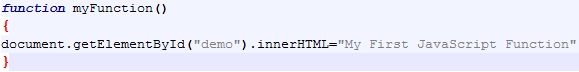
\includegraphics[width=\textwidth]{exemplo1}
	\end{minipage}
\end{figure}

\begin{figure}[!htbp]
	\caption{Exemplo 1 - Código em JavaScript formatado}
	\label{fig:Exemplo 1 - Código em JavaScript formatado}
	\centering%
	\begin{minipage}{.8\textwidth}
		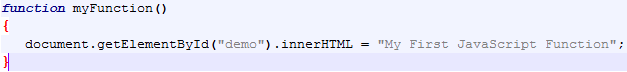
\includegraphics[width=\textwidth]{exemplo1_ok}
	\end{minipage}
\end{figure}

Nas Figuras \ref{fig:Exemplo 2 - Código em JavaScript não formatado} e \ref{fig:Exemplo 2 - Código em JavaScript formatado} temos novamente a comparação entre dois códigos que funcionam, porém o apresentado na Figura \ref{fig:Exemplo 2 - Código em JavaScript formatado} apresenta indentação, espaçamento nas atribuições e outras características que o tornam o código mais legível. 

\begin{figure}[!htbp]
	\caption{Exemplo 2 - Código em JavaScript não formatado}
	\label{fig:Exemplo 2 - Código em JavaScript não formatado}
	\centering%
	\begin{minipage}{.8\textwidth}
		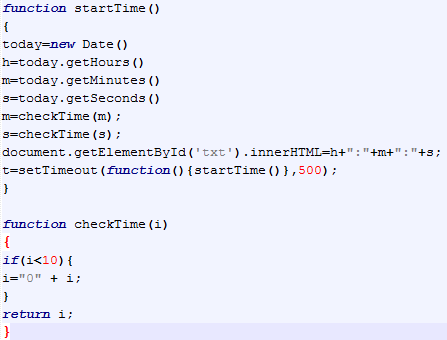
\includegraphics[width=\textwidth]{exemplo2}
	\end{minipage}
\end{figure}

\newpage

\begin{figure}[!htbp]
	\caption{Exemplo 2 - Código em JavaScript formatado}
	\label{fig:Exemplo 2 - Código em JavaScript formatado}
	\centering%
	\begin{minipage}{.8\textwidth}
		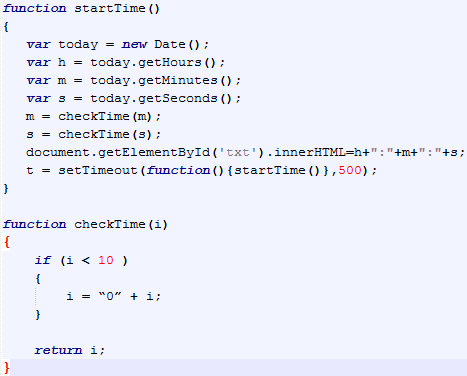
\includegraphics[width=\textwidth]{exemplo2_ok}
	\end{minipage}
\end{figure}

Os exemplos utilizados nesta sessão foram extraídos de \cite{W3Schools}.

\section{Ferramenta utilizada}

Para o desenvolvimento deste trabalho vamos utilizar a ferramenta \textit{ANTLT (ANother Tool for Language Recognition)}. O \textit{ANTLR} é uma ferramenta altamente utilizada no mercado e atualmente está na versão 4.2.2.

O \textit{ANTLR} foi escolhido pois com ele é possível realizar a analise léxica e sintática utilizando a mesma ferramenta. Além disso, apresenta uma arquitetura de funcionamento modular e amplamente documentada \cite{ANTLR}.

\bibliographystyle{sbc}
\bibliography{Tradutores_TrabalhoGB_-_Bernardo-Botelho_Yuri-Paludo}

\end{document}